\chapter{Defining a New Workload Model}

We believe that the workload model using constant-power used in prior work is too big of a simplification.
In a workload model that supports different phases, high-powered phases could, for example, be matched to carbon-intensity valleys.
Through this chapter, we will first conduct power measurements on a machine learning workload.
By that, we will infer a new model, \modelname{}, that can represent our findings of different power levels and the cost associated with resuming said workload.

\section{Power Measurements on Machine Learning Jobs}
\label{sec:power_measurements}

\paragraph{Test Environment}

The experiments are run on a personal computer, its specification being outlined in Table \ref{tab:measurement_environment}, the values being determined with the \verb|hwlist| and \verb|lshw| commands.

\begin{table}[h!]
    \centering
    \begin{tabular}{|c|c|}
    \hline
        Operating system & Ubuntu 24.04 LTS \\ \hline
        Kernel & Linux 6.8.0-39-generic \\ \hline
        CPU & AMD Ryzen 5 1600X Six-Core Processor \\ \hline
        Memory & 16GiB \\ \hline
        GPU & GeForce GTX 1070 \\ \hline
    \end{tabular}
    \caption{Environment parameters of the power measurements}
\label{tab:measurement_environment}
\end{table}

\paragraph{Measurement Tool}

As outlined in Chapter \ref{chap:backgroud}, multiple measurement options exist. 
As the HPI has the \emph{Microchip MCP39F511N Power Monitor} (henceforth called \emph{MCP}) on-site, one will be used as a physical measurement device.
The MCP is placed between the device to test and the wall-mounted power supply. 
A picture of it can be found in Figure \ref{fig:mcp}. 
It can report the current power consumption in 10 mW steps, each 5ms. 
The software used for reading out MCP data is \emph{pinpoint} \cite{kohler_pinpoint_2020}.
In our case, pinpoint us run on the device-to-test.

\begin{figure}
    \centering
    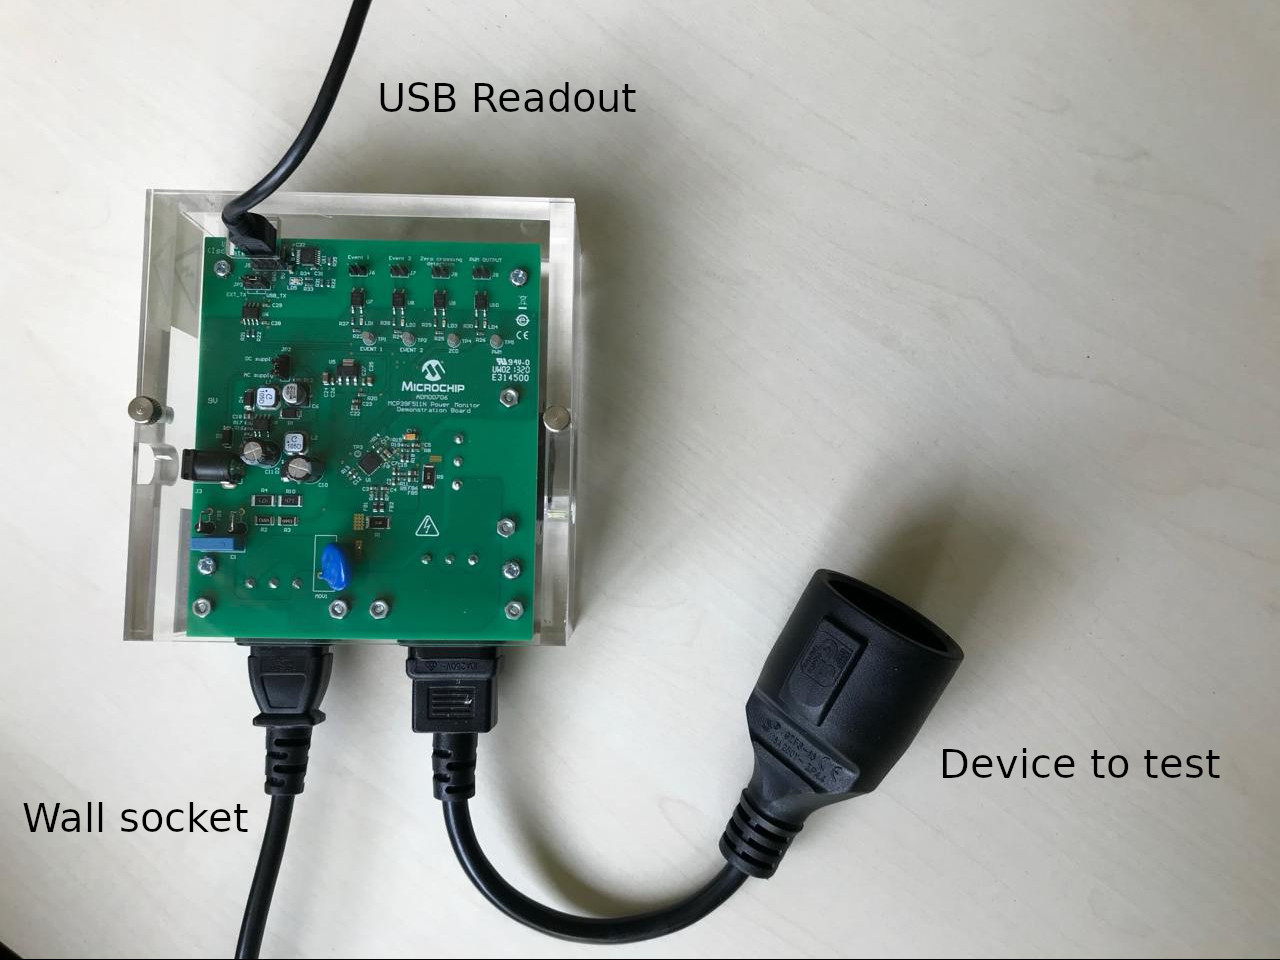
\includegraphics[width=200px]{images/mcp_graphic_design_is_my_passion.jpg}
    \caption[short]{The \emph{Microchip MCP39F511N Power Monitor}. It can be inserted between a devices power supply and the wall socket. Data is output via USB, which can be read by an external device or the device-to-test.}
    \label{fig:mcp}
\end{figure}


\paragraph{Benchmark}

Machine learning (ML) was used as the main motivation for suspend \& resume scheduling in prior works \cite {wiesner_lets_2021} and thus was also chosen by us to be measured and modeled. 

The concrete model and framework are secondary to our measurement. 
In our case, a small model, RoBERTa \webcite{web_distilbertdistilroberta-base_2024}, is chosen.
It is a natural language model, that due to its size generates fewer data points for processing, and allows faster iterations for the measurement script. 

There is a vast amount of machine learning frameworks. 
For our high-level model, the feature set of the framework only needed to support checkpointing, resuming, and some basic form of logging. 
A glance at the documentation of popular frameworks such as \emph{torch}, \emph{tensorflow}, and \emph{huggingface} shows that these features are commonly supported. 
With little bias towards any framework, huggingface was chosen.
The huggingface trainer supports callbacks, we modified a basic ML script to also log timestamped events when a training iteration, for example, starts or ends. 
These events are then saved into another \verb|.csv| file for each experiment.

\paragraph{Conducted Experiments}

A script, \verb|measure_roberta.sh|, was used to execute each experiment. 
On a high-level view, the following experiments were conducted: 

\begin{enumerate}
    \item \label{experiment:full}Run the whole program from start to finish
    \item \label{experiment:partial_checkpointed}Run it partially, checkpointing after some steps, sleeping, and resuming from that step
    \item \label{experiment:partial_checkpointed_aborted}Run it partially, checkpointing after some steps but aborting before the next checkpoint. Then resume as above.
    \item \label{experiment:startup_only}Run only the startup phase up until the ML starts
    \item \label{experiment:baseline}Do nothing, measure the system at rest
\end{enumerate}

Experiment \ref{experiment:full} gives a baseline for what the job looks like without suspending. 
Numbers \ref{experiment:partial_checkpointed} and \ref{experiment:partial_checkpointed_aborted} will be used to determine the overhead of checkpointing the job. 
Experiment \ref{experiment:startup_only} is used to validate the other ones, as it is a subset of the others. 
The last experiment is necessary to determine the baseline energy consumption of the environment.

To execute these experiments inside a repeatable bash script, additional command line parameters were added to the program. 
For example, a boolean parameter \verb|--resume_from_checkpoint| and an integer parameter \verb|--stop_after_epoch| are used for experiment \ref{experiment:full} to \ref{experiment:partial_checkpointed}. 
The way of conducting experiment \ref{experiment:startup_only} was to copy the script, and delete everything after the imports.

\paragraph{Creating Repeatable Measurements}

As this is being run on standard hardware on a standard operating system, all experiments are subject to noise. 
For example, \emph{Dynamic frequency and voltage scaling (DFVS)}, the OS technique of increasing CPU frequency for performance needs, adds power in an uncontrolled way. 
Also, background tasks may happen \emph{randomly}, increasing power usage. 
To reduce noise, we reduced the number of processes to a minimum.
We also used the Linux tool \verb|cpupower|, as shown in the snippet below, to set the CPU frequency to a set value of 3.6 GHz, which is the maximum frequency:

\begin{minipage}{\linewidth}
\begin{lstlisting}[language=bash, frame=single, numbers=none, caption={Used operating system information}, basicstyle=\ttfamily]
    MINFREQ=$(cpupower frequency-info --hwlimits | sed -n '1d;p' \
        | awk '{print $1}')
    MAXFREQ=$(cpupower frequency-info --hwlimits | sed -n '1d;p' \
        | awk '{print $1}')
    
    cpupower frequency-set --min ${MAXFREQ} &>/dev/null
    cpupower frequency-set --max ${MAXFREQ} &>/dev/null

    # ... conduct experiments

    cpupower frequency-set --min ${MINFREQ} &>/dev/null
    cpupower frequency-set --max ${MAXFREQ} &>/dev/null
\end{lstlisting}
\label{listing:setting_cpu_frequency}
\end{minipage}

As machine learning makes use of available GPUs, its frequency should also be similarly set to a defined value. 
NVIDIA provides a guide on how to conduct power measurements on GPUs~\webcite{web_nvidiapower}.
Our used GPU, the NVIDIA GTX 1070, is not capable of fixing the frequency as of the time of conducting these experiments. 
While it is supposed to be possible, there seems to currently be driver issue preventing this \webcite{web_powerlimitissue}.
Thus, the frequency of the GPU was not fixed. 
To reduce the effect of frequency scaling here, the time between experiments was increased generously so that any impact from such scaling reoccurs throughout each run, reducing dependencies between runs.

For the training, data is downloaded and saved, which is however deleted before the next experiment. 
The Python process is also not kept between runs, forcing a reload of any libraries.

\paragraph{Conducting each Experiment}

Each experiment was repeated ten times to be able to average out noise later.
Between each run, there is a \verb|sleep| period of 10 seconds and one of two minutes in the partial executions. 
Additionally, \verb|pinpoint|'s feature of measuring before and after the actual program-to-test was used. 
This leads to a period of 30 seconds being measured around the program execution. 
Plotting these additional time frames gives a quick visual indicator of whether experiments are sufficiently isolated from each other, ergo when the power draw is at the baseline as the actual program starts.

\newpage
\paragraph{Collected Data}

For each experiment, a named and timestamped folder is created in the \verb|/power-measurements| folder of our repository. 
Each folder then holds a \verb|.csv| with pinpoint's timestamped power measurements. 
The added timestamped logging is saved into another \verb|.csv|. 
On the way to the final measurements, we plotted each experiment early and visually checked if there were any obvious errors or mistakes.

\paragraph{Determining the Baseline Power Draw}

A sample run of the baseline experiment is shown in Figure \ref{fig:plot_baseline}.
The blue dots represent each data point. The red line is a smoothed Gaussian trend line with $\sigma = 2$. 

\begin{figure}[H]
    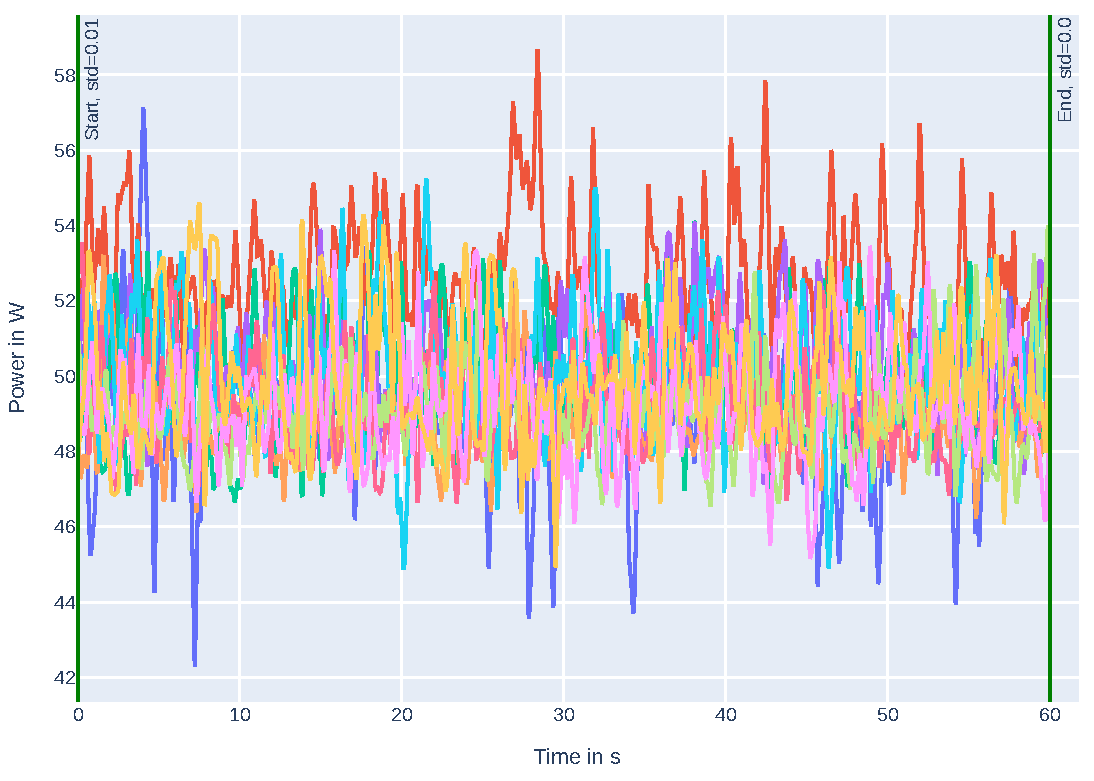
\includegraphics[width=\linewidth]{power-measurements/stacked_plots/sleep_0714.pdf}
    \caption{In the baseline experiment of measuring the system at rest, the average power draw is about 50 W. The black lines are Gaussian smoothed trend lines with $\sigma = 2$.}
    \label{fig:plot_baseline}
\end{figure}

Across all ten runs, the average baseline power draw is calculated via the mean of all data points. This comes out as an average of 49.8 W with a standard deviation of 4.4 W.

The baseline power draw will be less interesting going further but will put perspective on the other experiments. 
The standard deviation gives a broad idea of the environment noise.

\paragraph{The Full Run}

For the unsuspended machine learning, Figure \ref{fig:plot_full_stacked} shows the stacked trend lines of the 10 different runs.
A single sample run is provided in Figure \ref{fig:plot_full}. 
The times of each event occurred within a standard deviation of less than 1 second.
Thus, for simplicity's sake, we refrained from doing a more elaborate statistical analysis of the different runs as the visual check of them being very similar seemed enough.

\begin{figure}[H]
    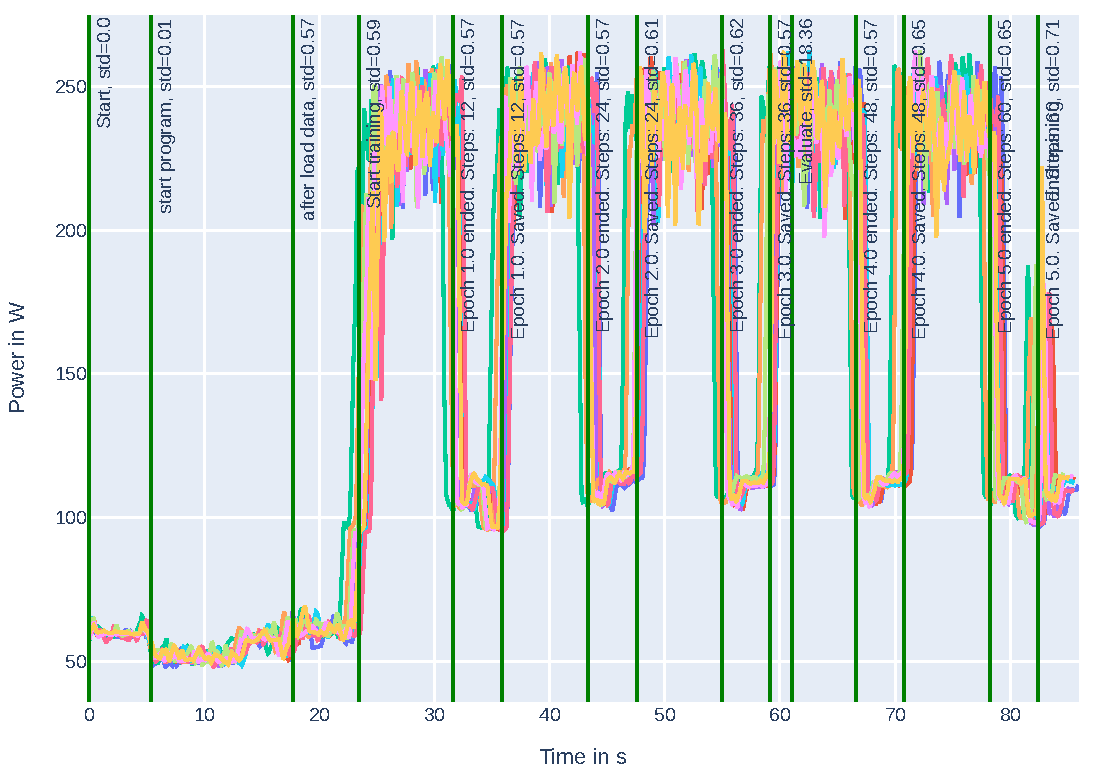
\includegraphics[width=\linewidth]{power-measurements/stacked_plots/roberta_full_0714.pdf}
    \caption{Each black line is a Gaussian-smoothed trend line of a run. We stack all 10 measurements into one time series, showing that each is similar to the others. The background represents our derived phases. Their borders are when our manually added events occurred on average. The timestamp of each event had a standard deviation of less than 1 second, meaning that there was little variation.}
    \label{fig:plot_full_stacked}
\end{figure}

The main takeaways from these measurements are:
\begin{enumerate}
    \item There is a long (about 25\%) start-up phase, which is spent in starting Python, loading libraries, and setting up the training data.
    \item There are periodical work phases; a high-power training phase is followed by low-power evaluation phase and a low-power checkpointing.
    \item A higher variance in measurements occurs during the training phases in comparison to the others.
\end{enumerate}

This already shows, that improvements upon the constant-power model used in \cite{wiesner_lets_2021} are possible. 
For example, in this case, the start-up phase has a much lower power-draw than the work-phase.

\begin{figure}[H]
    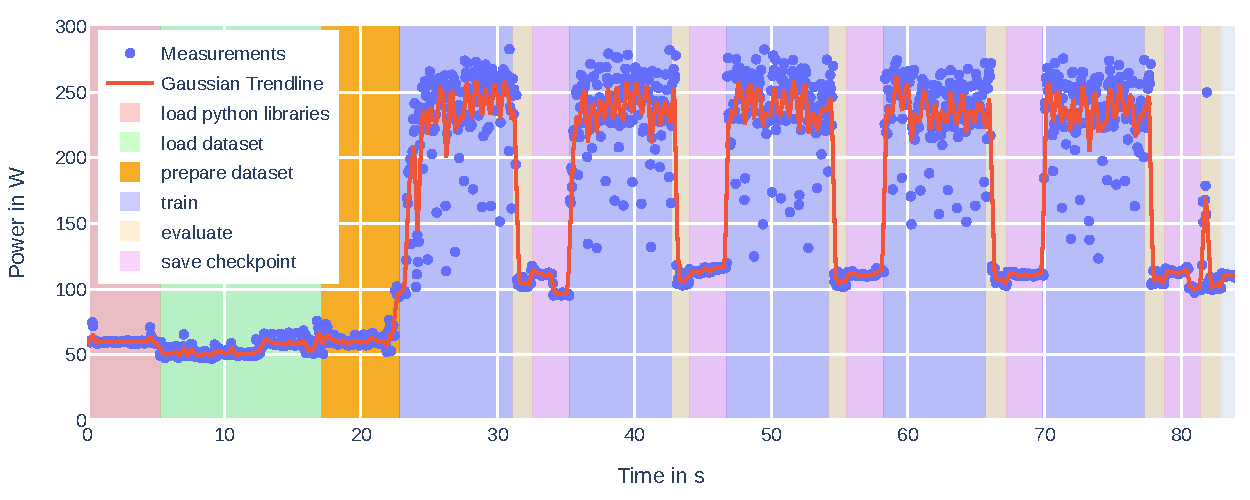
\includegraphics[width=\linewidth]{power-measurements/measurements_roberta_full_0714010405/plot.pdf}
    \caption{Sample run of the full run experiment, the background indicates each phase. These phases are derived from our manually added logging.}
    \label{fig:plot_full}
\end{figure}

\newpage
\paragraph{Results of Checkpoint and Restore}

Similarly to before, results will be discussed using the stacked plots of Figures \ref{fig:plot_partial_saved_stacked} and \ref{fig:plot_partial_saved_continue_stacked}.

\begin{figure}[H]
    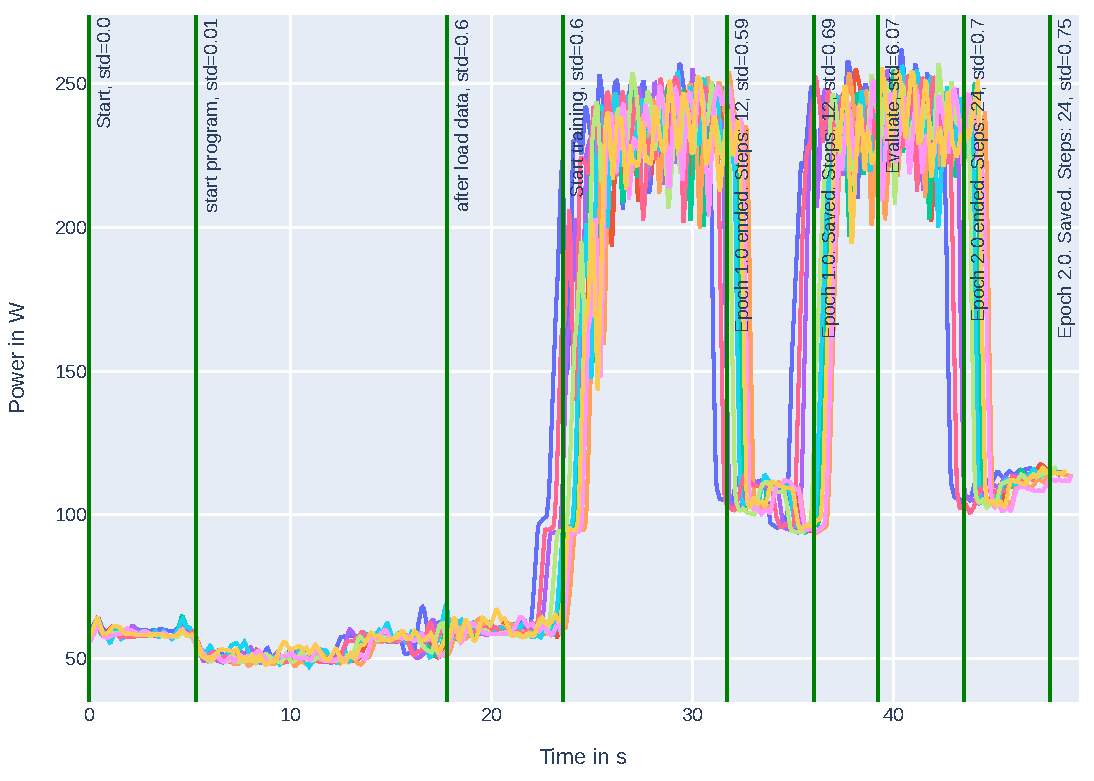
\includegraphics[width=\linewidth]{power-measurements/stacked_plots/roberta_stop_after_saving.pdf}
    \caption{Stacked trend lines of the experiment for stopping after the second epoch}
    \label{fig:plot_partial_saved_stacked}
\end{figure}

\begin{figure}[H]
    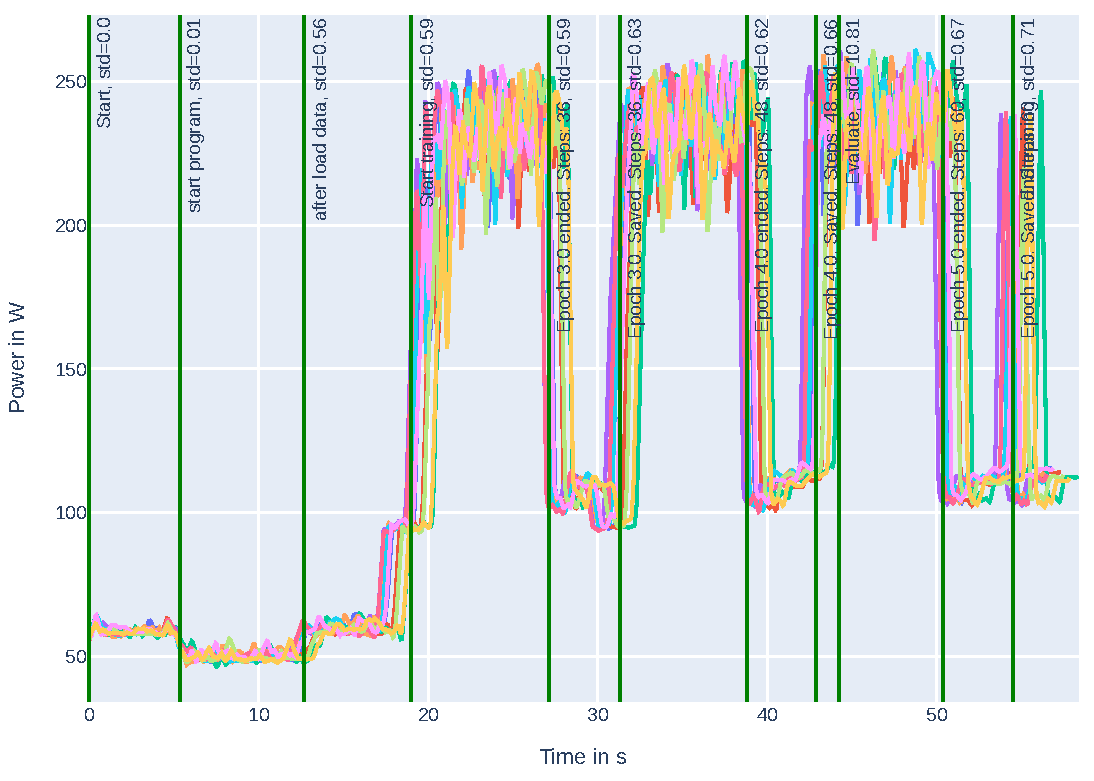
\includegraphics[width=\linewidth]{power-measurements/stacked_plots/roberta_continue_after_saving.pdf}
    \caption{Stacked trend lines of the experiment for continuing after the second epoch}
    \label{fig:plot_partial_saved_continue_stacked}
\end{figure}

Here we can observe that:

\begin{enumerate}
    \item The amount of work done is the same. 
    Similarly to the full-run experiment, the ML training still takes the full 5 epochs and has the same work-phases
    \item There is no overhead from checkpointing itself, as the checkpoints are being created regardless of them being resumed from later.
    \item Resuming the jobs results in an added start-up phase. This phase is slightly shorter by a few seconds than the ones in the full runs, perhaps due to not needing to download the dataset again.
\end{enumerate}

\newpage
\paragraph{Results of Aborting the Checkpoint and Resuming}

Unlike the previous experiment, where the training is stopped as soon as a checkpoint is created, this time the program will be stopped just before a checkpoint is created (in this case just the second checkpoint would be saved). 
Ideally, this represents the maximum overhead from a suspend \& resume strategy. 
Again, the results are visualized in Figures \ref{fig:plot_partial_abort_stacked} and \ref{fig:plot_partial_abort_continue_stacked}. 

\begin{figure}[H]
    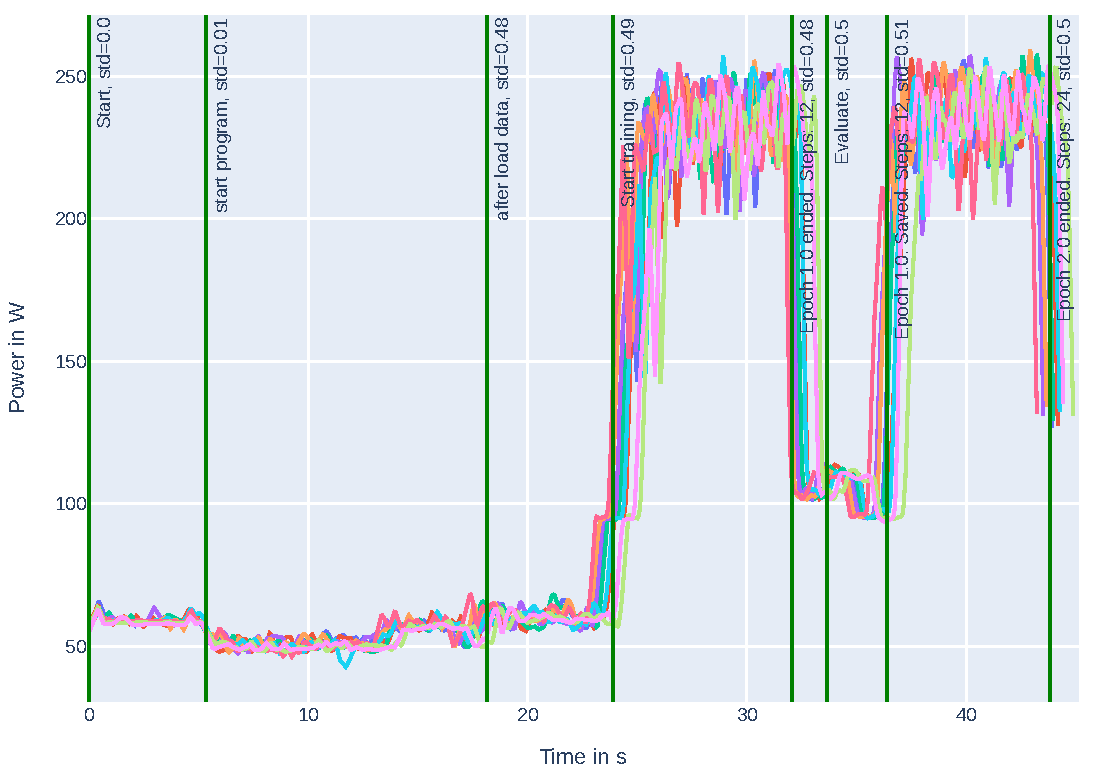
\includegraphics[width=\linewidth]{power-measurements/stacked_plots/roberta_stop_without_saving.pdf}
    \caption{Power draws of the ML up until stopping after epoch 2}
    \label{fig:plot_partial_abort_stacked}
\end{figure}

\begin{figure}[H]
    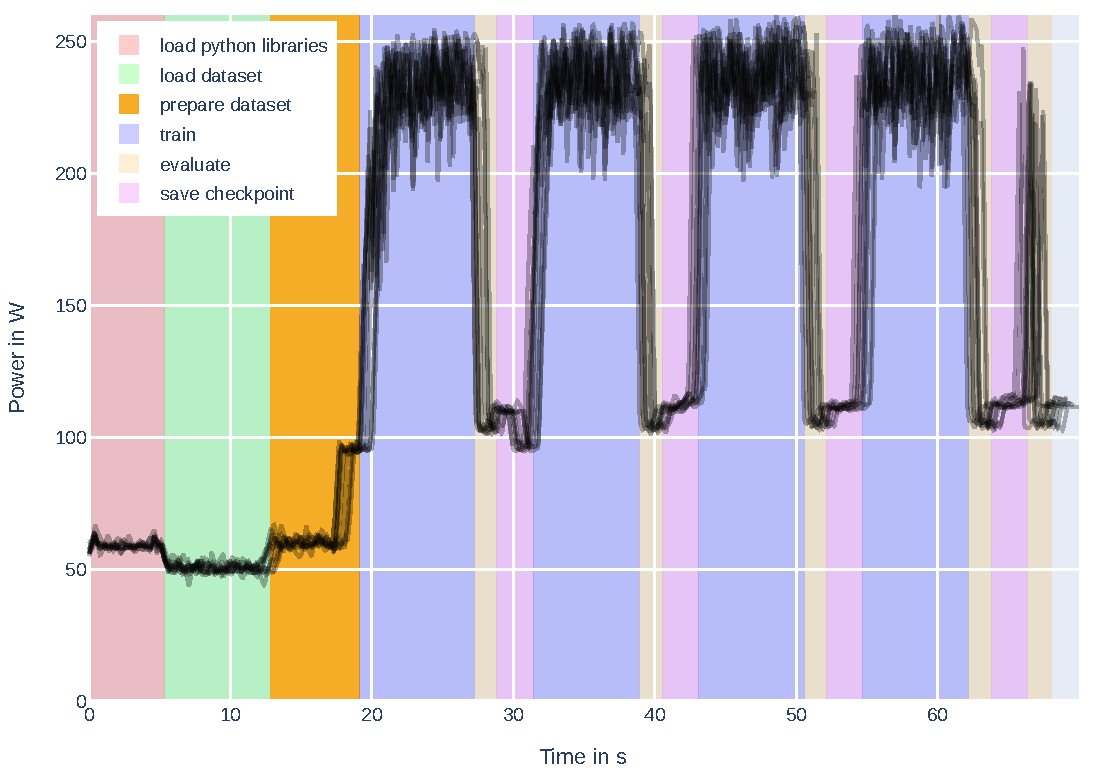
\includegraphics[width=\linewidth]{power-measurements/stacked_plots/roberta_continue_after_not_saving.pdf}
    \caption{Power draws after continuing from the second checkpoint}
    \label{fig:plot_partial_abort_continue_stacked}
\end{figure}

Attention should be paid that,

\begin{enumerate}
    \item The behavior of the repeated start-up phase is kept
    \item There is now a full additional training and evaluation phase added to the overall work, the aborted checkpoint is also repeated.
\end{enumerate}

While this may sound artificial, it could happen in environments where the interaction between the scheduler and the job is not well orchestrated, for example in an environment where jobs are stopped \emph{at random} like in a cloud spot instance. 
The average overhead from stopping the job at random vs. stopping after a checkpoint will likely fall at half the cost of an epoch.

\paragraph{Calculating the Energy Costs of each Run}

The energy costs of each experiment are contained in Table \ref{tab:experiment_overhead}. 
Showing that there indeed is an overhead created from suspending at different parts of the program execution.

\begin{table}[h!]
    \centering
    \begin{tabular}{|c|c|c|}
    \hline
        Experiment & average energy cost & standard deviation \\ \hline
        \ref{experiment:full}, whole run &  12.97 kJ & 0.04 \\ \hline
        \ref{experiment:partial_checkpointed}, suspend after checkpoint and resume &  13.94  kJ & 0.1 \\ \hline
        \ref{experiment:partial_checkpointed_aborted}, abort early and resume &  15.72 kJ & 0.07 \\ \hline
    \end{tabular}
    \caption{Energy costs of the different experiments. Unlike the no-overhead assumption in prior work, we can show that suspending a workload does carry overhead.}
\label{tab:experiment_overhead}
\end{table}

\section{Introduction of \modelname} \label{sec:improving_the_model}

Now that we know what a high-level job looks like, we can pick it apart and reduce the real-world measurements of one program to a more generic model. 
Summarizing the findings from the previous paragraphs; it was shown that 

\begin{itemize}
    \item The given job has phases that have different power draws
    \item Checkpointing \& resuming carries overhead in the form of startup costs and possible wasted work.
\end{itemize}

We thus propose \modelname{}: a model combining startup, work, and phases.
Its definition is given the form of the Python implementation in Listing \ref{listing:model_python}.

\begin{minipage}{\linewidth}
\begin{lstlisting}[language=python, frame=single, numbers=none, caption={Definition of \modelname{} as a Python class}, basicstyle=\ttfamily, label={listing:model_python}]
class Stawp(TypedDict):
    startup: List[Phase]
    work: List[Phase]
    
class Phase(TypedDict):
    name: str
    duration: float
    power: float
    is_checkpoint: NotRequired[bool]   
\end{lstlisting}
\end{minipage}

Some simplifications are made: the duration of each phase is well known and the power per phase is constant. 
Phases can also be named for later reference.
These phases essentially define a step function, i.e. a piecewise constant function.
Unlike a traditional step function, the start- and endpoints of each piece are encoded implicitly by the previous phases.
With this, a simple time-to-power function can be defined, that looks up the input time by traversing the phases in order.

Initially, we considered allowing any expression instead of a constant value for power and then using Python's \verb|evaluate()| to e.g. allow a function-per-phase model.
In Section \ref{sec:checkpoint_resume_lp}, having a rather restrictive step function will be of advantage, however.

\paragraph{Fitting \modelname to RoBERTa}

We use the following pseudocode: 

\begin{minipage}{\linewidth}
    \begin{lstlisting}[frame=single, numbers=left, caption={Pseudocode for turning RoBERTa's power measurements into \modelname}, basicstyle=\ttfamily, label={listing:fitting_swap}]
phases = []
iterate with event_1 and event_2 pairwise through the events:
        # do this in respect to each run:
        phase_measurements = measurements between pair of events
        phase_power = average of phase_measurements
        phase_duration = 
            average time of all event_2
            - average time of all event_1
        phases += {phase_duration, phase_power, name of event_2}
        
manually reorder phases into startup and work
    \end{lstlisting}
\end{minipage}

In line 4 we query each run for phase-associated measurements based on that runs event timings. 
The durations of the phases are calculated similarly by taking the average time the logging occurred during the measurements.

Using this strategy on the ten complete runs results in Figure \ref{fig:model_overlaid}, which shows the derived model in black with the previous Figure \ref{fig:plot_full_stacked} in less opacity. 
The startup phase looks well approximated, visually however there is some error during the work phases.
The training phases each have a high variance, which is not captured by the constant power approximation. After each training  phase, the power goes down seemingly linearly, which is also approximated by the constant.
One notable point: this model is a superset of the previous constant-no-overhead model used in the related work.
Previous jobs can be modeled with just one phase of work, resulting in constant power over its execution. Leaving the startup phases empty creates no overhead on resuming.

\paragraph{Model Error Analysis}

To analyze the error of this model, we cross-validated the power's RMSE and the total energy using \verb|scikit-learn|'s \verb|LeaveOneOut| strategy. 
The first one gives a measure of the model's accuracy on a short-time (sub-second) scale, the latter tells the long-time (whole job) scale accuracy of the model.

Each of the ten runs is taken as the ground truth while the other nine are used to create the model. 
The results are the following: the power between the prediction and remainder has an RSME of 39.3 W while the difference in total energy is calculated as -0.1 kJ. 

Interpreting this, it seems that the model performs poorly as a predictor of the exact power used at some time point as the RMSE is rather large (think of the maximum power drawn being about 250W). 
However, in the context of carbon-aware scheduling, this should not be too big of an issue as the time frames for carbon emissions are orders of magnitudes larger. 
For example, Electricitymaps has a resolution of 1 hour for carbon emissions intensities. 
The high error likely comes from the high variance during the training phases which is not captured in the model.

The total energy predicted by the model is very close to the actual real-life experiment, this should mean that the total carbon calculated on the model should also be close to the carbon emitted by the real program.

\begin{figure}
    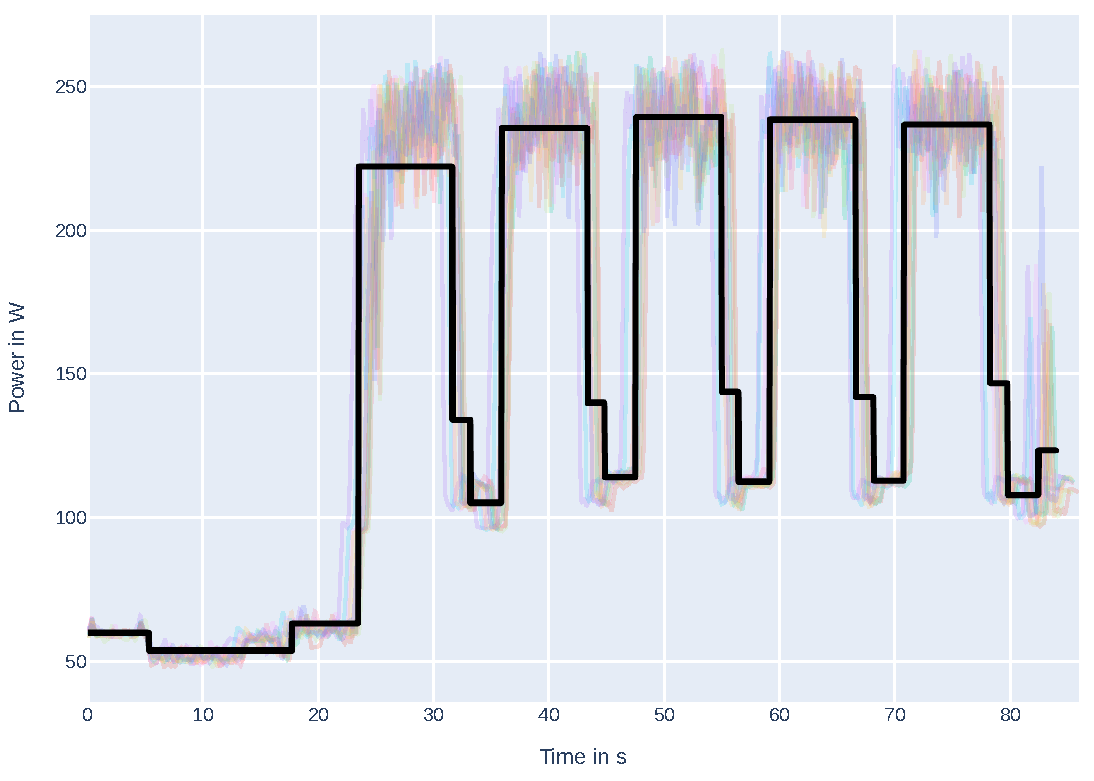
\includegraphics[width=\linewidth]{power-measurements/model_overlaid.pdf}
    \caption{\modelname{} vs RoBERTa. The black line is the new model we propose and the others lines are individual runs. Each of \modelname{}'s phases is the result of averaging the runs measurements between two events. The length of a phase is similarly derived from the average time of each event.}
    \label{fig:model_overlaid}
\end{figure}
